\documentclass[10pt,a4paper]{report}
\usepackage[utf8]{inputenc}
\usepackage[portuguese]{babel}
\usepackage[T1]{fontenc}
\usepackage{amsmath}
\usepackage{amsfonts}
\usepackage{amssymb}
\usepackage{graphicx}

\usepackage{titlesec}
\usepackage{termcal}

\graphicspath{{./img/}}

\author{Lucas Lopes Costa}
\title{Relatório}

\titleformat{\chapter}{\normalfont\huge}{\thechapter.}{20pt}{\huge\bf}

\begin{document}
\chapter{Resumo}

Neste trabalho desenvolvemos uma versão simplificada de um jogo de computador bastante conhecido, o Campo Minado. Tendo em vista a finalidade didática da execução deste projeto, buscamos utilizá-lo como plataforma para pôr em prática variadas técnicas e ferramentas de planejamento e desenvolvimento de software. O projeto foi executado por uma equipe de quatro alunos no período de 2 de junho à 1 de julho.

\chapter{Introdução}

Neste trabalho desenvolvemos uma versão simplificada de um jogo de computador bastante conhecido, o \textbf{Campo Minado}. Tal jogo, conhecido também como \textbf{Minesweeper}, tem origens na década de 60, e consiste de um tabuleiro, inicialmente coberto, onde aleatóriamente são semeadas bombas, e demarcadas dicas numéricas à respeito do número de bombas nas redondezas de uma casa. O jogador deve a cada jogada indicar uma casa, e marcá-la como minada, ou ``pisar'' sobre a mesma, revelando seu conteúdo e, se vazia, de sua vizinhança. O objetivo é demarcar a localização de todas as bombas presentes no tabuleiro, utilizando as dicas reveladas, sem que se ``pise'' sobre uma casa minada.

Tendo em vista a finalidade didática da execução de tal projeto, buscamos utilizá-lo como plataforma para o exercício de variadas práticas em planejamento e desenvolvimento de software. Com isso estabelecemos um particionamento de etapas e tarefas na equipe, seccionando o projeto em módulos, cada um sob a responsabilidade de um integrante. Debatemos e definimos também um conjunto específico de ferramentas a ser utilizado, visando facilitar a comunicação e o desenvolvimento em grupo.

Dividiu-se a execução do projeto em três fases principais, \textbf{Planejamento}, \textbf{Desenvolvimento} e \textbf{Teste}.

\chapter{Planejamento}
Nesta primeira fase, que representa o início do projeto como um todo, o foco esteve em definir as bases para as fases de desenvolvimento e teste, o que inclui a determinação de um \textbf{Cronograma}, a determinação de uma \textbf{Estrutura do Projeto}, a divisão das tarefas de desenvolvimento, e a escolha das \textbf{Ferramentas} em software utilizadas pela equipe.
\section{Cronograma}
Iniciando no dia 2 de junho, organizamos a primeira reunião da equipe de projeto, onde determinamos os primeiros tópicos a serem determinados, e a partir destes formulamos o cronograma apresentado abaixo.
\begin{calendar}{6/1/16}{5}
\setlength{\calboxdepth}{.3in}

\calday[Quarta-feira]{\classday}
\calday[Quinta-feira]{\classday}
\calday[Sexta-feira]{\classday}
\skipday\skipday
\calday[Segunda-feira]{\classday}
\calday[Terça-feira]{\classday}

\caltexton{1}{Início da Fase de Planejamento}
\caltexton{2}{Reunião:\\Cronograma e estrutura do projeto}
\caltexton{4}{Reunião:\\Estrutura do projeto e ferramentas}
\caltexton{5}{Reunião:\\Estrutura do projeto}
\caltexton{6}{Reunião:\\Estrutura do projeto}
\caltexton{9}{Início da Fase de Desenvolvimento}
\caltexton{10}{Reunião:\\Escrita de código em grupo}
\caltexton{18}{Primeiro Build funcional}
\caltexton{19}{Início da Fase de Teste}
\caltexton{22}{Conclusão do Projeto}
\end{calendar}
\section{Estrutura do Projeto}
Durante as primeiras reuniões um dos principais tópicos foi a Estrutura do Projeto como um todo. Já que a idéia dominante nas discussões era a de como seria a secção do projeto e a divisão das tarefas de desenvolvimento, e já que este determina como será escrito o software todo, este mostrou-se como o tópico mais importante de toda a primeira fase da execução do projeto.

Logo no início, ficara decidido que o projeto teria uma estrutura modular, com unidades de código bem delimitadas, e relacionadas entre si por interfaces pré-definidas, de maneira que o código seja o mais flexível possível, mantendo ainda uma alta independência de implementação.

Estas escolhas de design direcionaram o projeto para um estilo próximo à Programação Orientada à Objetos e a Programação Modular. Com isso, as posteriores reuniões foram reservadas apenas à determinação dos módulos e de suas interfaces de código. Ao fim 

\begin{figure}[h]
\centering
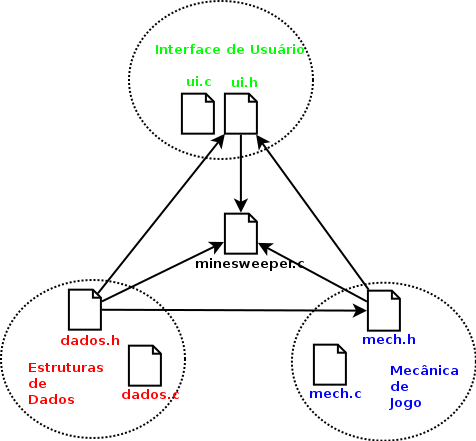
\includegraphics[width=0.5\textwidth]{diagrama.png}
\caption{Módulos e Arquivos do Projeto}
\end{figure}
\section{Ferramentas}
T
\chapter{Desenvolvimento}
T
\section{Execução}
T
\chapter{Conclusão}
T
\end{document}